\chapter{Metodologie}
In questo capitolo verranno delineate nel dettaglio le varie metodologie scelte per la realizzazione della comparazione fra alcune strategie di addestramento continuo triviali applicate ai dataset di Human State Monitoring presentati nel precedente capitolo.\\\\
In particolare, nella sezione 3.1 vengono delineate nel dettaglio le metriche prese in considerazione per comparare le metodologie scelte, nella sezione 3.2 viene presentata la metodologia di addestramento utilizzata come base di confronto e infine, nella sezione 3.3, vengono descritte nel dettaglio le metodologie di addestramento continuo selezionate nell'ambito di questa tesi.
\section{Metriche}
Per poter confrontare fra loro le diverse strategie, fin da subito è apparsa chiara la necessità di metriche che misurassero con precisione alcune caratteristiche fondamentali delle metodologie di addestramento continuo, in particolare: l'accuratezza sul test set, l'accuratezza media sulle classi e i \textit{forward} e \textit{backward transfer} per poter misurare l'impatto della nuova conoscenza sulla conoscenza precedentemente appresa e su quella ancora da acquisire.
\subsection{Accuratezza}
Con "accuratezza" si intende la misura della percentuale di previsioni corrette che il modello di Machine Learning ottiene su un test set, cioè un insieme di dati a cui il modello non è stato esposto durante le sessioni di addestramento.\\
Per poter misurare l'accuratezza su un insieme di dati, l'API di TensorFlow mette a disposizione un comando che valuta un modello di Machine Learning applicato ai dati passati come parametro:
\begin{lstlisting}[style = myPython]
model.evaluate(Xtest, ytest)
\end{lstlisting}
Questa chiamata ritorna il valore assunto dalla funzione di loss al termine della valutazione e le metriche che vengono specificate durante la compilazione del modello. Compilando il modello con il seguente comando
\begin{lstlisting}[style = myPython]
model.compile(loss = 'categorical_crossentropy', optimizer = opt, metrics = ['accuracy'])
\end{lstlisting}
otterremo un modello la cui funzione di loss è la cross-entropia categorica, usata per modelli che devono classificare dati appartenenti ad una sola classe fra diverse disponibili, e come metrica aggiuntiva richiediamo l'accuratezza. Così facendo, con
\begin{lstlisting}[style = myPython]
model.evaluate(Xtest, ytest)[1]
\end{lstlisting}
otteniamo la misura dell'accuratezza che il modello \texttt{model} ottiene sul test set composto dai dati \texttt{Xtest} e dalle etichette \texttt{ytest}.\\\\
La misura di accuratezza indicata nei risultati è l'accuratezza media ottenuta dal modello durante le varie sessioni di addestramento.
\subsection{ACC, FWT e BWT}
Queste tre metriche sono state tratte e adattate dalla pubblicazione \textit{Gradient Episodic Memory for Continual Learning}$^{\cite{DBLP:journals/corr/Lopez-PazR17}}$, e si basano sulla costruzione di una matrice $R \in \mathbb{R}^{E\times T}$. Con $T$ si indica il numero di classi del problema in esame, e ogni volta che il modello finisce una sessione di addestramento tra le $E$ che vengono eseguite si va a valutare la sua \textit{test performance} su tutte le $T$ classi. Così facendo, si calcolano le $R_{i,j}\in R$ valutazioni dell'accuratezza del test di classificazione del modello sulla classe $t_j$ dopo aver osservato gli esempi della $i$-esima sessione di addestramento. Inoltre, una volta creato il modello con una inizializzazione dei pesi casuale si calcola $\overline{b}$, valutazione delle accuratezza nei test sui vari task.\\
Possiamo ora definire le tre metriche:
\begin{itemize}
    \item[-] \textbf{ACC}, \textit{Accuracy} o accuratezza
        \begin{equation}\label{eq:fun_acc}
            ACC = \frac{1}{T}\cdot\sum_{i=1}^T R_{E,i}
        \end{equation}
    Va a misurare l'accuratezza del modello su tutti le $T$ classi a fine addestramento
    \item[-] \textbf{BWT}, \textit{Backward Transfer} o trasferimento all'indietro
        \begin{equation}\label{eq:fun_bwt}
            BWT = \frac{1}{T-1}\cdot\sum_{i=1}^T\left(\frac{1}{E}\sum_{j=1}^E R_{E,i} - R_{j,i}\right)
        \end{equation}
    Valuta l'influenza che ha una sessione di apprendimento sulle precedenti, valutando l'impatto che ha avuto sulle valutazioni dell'accuratezza in fase di test. Si ha un BWT positivo quando una sessione di addestramento migliora l'accuratezza delle precedenti già valutate, mentre un valore negativo indica che la sessione di addestramento ha deteriorato l'accuratezza che si otteneva grazie alla precedente conoscenza. Non è significativo parlare di BWT durante la prima sessione di addestramento.\\
    Un BWT fortemente negativo evidenzia il verificarsi del fenomeno del \textit{catastrophic forgetting}.
    \item[-] \textbf{FWT}, \textit{Forward Transfer} o trasferimento in avanti
        \begin{equation}\label{eq:fun_fwt}
            FWT = \frac{1}{T-1}\cdot\sum_{i=1}^T\left(\frac{1}{E}\sum_{j=1}^E R_{j,i} - \overline{b}_i\right)
        \end{equation}
    Serve per misurare l'influenza che la sessione di apprendimento ha sulla conoscenza ancora da apprendere. In particolare, un FWT positivo è possibile quando il modello è in grado di realizzare lo \textit{zero-shot} learning, cioè di apprendere informazioni sui task futuri senza essere esposto ad esempi da apprendere, per esempio sfruttando la struttura interna della conoscenza in caso di task simili.\\
    Non è significativo parlare di FWT durante l'ultima sessione di addestramento.
\end{itemize}
Tra queste tre, quella senza dubbio più interessante ai fini dell'esperimento è il BWT. Diventa particolarmente importante evitare gli scenari che portano al \textit{catastrophic forgetting}: nel nostro caso, uno scenario simile porterebbe a dimenticare esempi di HSM passati e a far sì che il modello si basi solamente sull'esperienza recente, rischiando di dimenticare importanti esempi passati di stati d'animo e di conseguenza a non saper più riconoscerli correttamente.\\\\
Più grandi sono queste metriche, migliore è il comportamento del modello in esame. A parità di ACC, si preferisce il modello con maggior BWT e FWT che denoterebbe un miglior trasferimento della conoscenza attraverso i task e le sessioni di training.
\subsection{Altre metriche}
Le altre metriche raccolte durante gli esperimenti sono le seguenti:
\begin{itemize}
    \item[-] \textbf{Numero di epoche} medio, e deviazione standard\\
    Questa misurazione fornisce una indicazione sul tempo di convergenza delle reti neurali selezionate sui dati, così da poter stimare le loro prestazioni su hardware diversi da quello di test.
    \item[-] \textbf{Tempo di addestramento} medio, e deviazione standard\\
    Gli esperimenti sono eseguiti su un personal computer comune, sfruttando le ottimizzazioni messe a disposizione dall'utilizzo di una GPU per i calcoli. Nello specifico, le computazioni sono state eseguite su una macchina che montava una GPU nVidia GeForce GTX 1070 con 6 Gb di memoria dedicata, una CPU Intel i5 3570 e 12 Gb di RAM.\\% CUDA 10.1 https://ai-benchmark.com/ranking_deeplearning.html
    Il tempo di addestramento è calcolato come la media dei tempi impiegati delle varie sessioni di addestramento.
    \item[-] \textbf{Quantità di memoria} media\\
    Metrica utile per valutare l'impatto sulla memoria del sistema che andrà poi a utilizzare il modello addestrato. Un elevato consumo di memoria può portare alla esclusione di dispositivi portatili o con specifiche particolari.
\end{itemize}

\section{Baseline: l'addestramento offline}
L'approccio classico all'addestramento di un modello di Machine Learning avviene raccogliendo i dati di addestramento e sottoponendoli al modello in una singola sessione di addestramento. Questa metodologia è statica e produce un modello che sui futuri dati si comporterà tanto meglio quanto essi saranno simili ai dati di addestramento.\\
La scelta di usare questa metodologia classica come baseline è stata guidata dal principio che, avendo tutti i dati a disposizione in una sola volta, la rete neurale risultante dovrebbe ottenere le migliori prestazioni possibili sul test set una volta che questo viene sottoposto, e quindi fornisce un "limite superiore" all'accuratezza delle metodologie continue. Una strategia di addestramento continuo è tanto migliore quanto più si avvicina alle performance che la stessa rete neurale otterrebbe se venisse addestrata su tutti i dati in maniera offline o, se possibile, quando la supera.\\\\
L'addestramento offline è quindi realizzato seguendo il seguente pseudo-algoritmo, applicabile sia a WESAD che ad ASCERTAIN:
\begin{enumerate}
    \item \textbf{Creare e compilare la rete neurale} che verrà poi addestrata.\\
    La creazione della rete neurale, attraverso la API Sequential di TensorFlow, è analoga per entrambi i dataset a meno della struttura interna. L'esempio seguente è tratto dall'addestramento offline per WESAD, e costruisce una rete neurale con due layer da 18 unità GRU e un layer output da 4 unità, corrispondenti alle 4 classi del dataset.
    \lstinputlisting[style=myPython, firstnumber=22, firstline=22, lastline=30]{code/wesad_totaltrain.py}
    \item \textbf{Caricare il dataset}, composto da training set e test set.\\
    Come precedentemente spiegato, i dataset sono divisi in training set e test set, e il training set è ulteriormente diviso fra i soggetti dei due studi. In entrambi i casi quindi, per quanto riguarda la metodologia offline, viene caricato il test set così come viene fornito, mentre il training set è realizzato concantenando fra loro i dati di tutti i soggetti. Esempio, sempre tratto da WESAD:
    \lstinputlisting[style=myPython, firstnumber=35, firstline=35, lastline=47]{code/wesad_totaltrain.py}
    \lstinputlisting[style=myPython, firstnumber=51, firstline=51, lastline=52]{code/wesad_totaltrain.py}
    Il training set è ulteriormente diviso in training set e validation set, utilizzato per monitorare l'andamento dell'addestramento e implementare la fermata anticipata dell'addestramento:
    \lstinputlisting[style=myPython, firstnumber=56, firstline=56, lastline=56]{code/wesad_totaltrain.py}
    \item \textbf{Addestramento} e risultati.\\
    Una volta preparato il dataset, si può dare il via all'addestramento. Prima di esso si preparano, sempre grazie all'API di TensorFlow, le due callback usate durante gli esperimenti: la creazione di grafici attraverso TensorBoard e la fermata anticipata in base all'andamento del valore della funzione di loss sul validation set:
    \lstinputlisting[style=myPython, firstnumber=59, firstline=59, lastline=68]{code/wesad_totaltrain.py}
    I risultati sono poi proiettati in output sul terminale:
    \lstinputlisting[style=myPython, firstnumber=70, firstline=70, lastline=73]{code/wesad_totaltrain.py}
\end{enumerate}
La metodologia offline, come visto, è immediata e grazie alle API di TensorFlow anche semplice da implementare. Essa è stata utilizzata anche per poter selezionare la rete neurale usata per il dataset relativo, una per WESAD e una per ASCERTAIN e che è poi stata usata su ciascun esperimento, in base all'accuratezza finale raggiunta.

\section{Metodologie di Addestramento Continuo}
Al centro di questo progetto ci sono le metodologie di addestramento continuo. Ne sono state selezionate alcune: 3 tecniche di replay e 2 tecniche che non sfruttano esempi già visti.\\\\
Per realizzare il flusso di dati necessario a implementare una strategia di addestramento continuo, le quali richiedono che i dati di addestramento non siano subito tutti disponibili ma che lo diventino nel tempo, i soggetti di entrambi i dataset sono stati mantenuti divisi per soggetto e raggruppati a coppie, per poi essere sottoposti all'addestramento della rete neurale una coppia per volta. Le tabelle \ref{tab:coppiewesad} e \ref{tab:coppieascertain} mostrano la suddivisione a coppie rispettivamente per il dataset WESAD e il dataset ASCERTAIN.
\begin{table}[h]
    \parbox{.45\linewidth}{
    	\begin{center}
    		\begin{tabular}{l|c}
    		     \textbf{Sessione} & \textbf{Coppie}\\
    		     \hline
    		     1 & S2, S3 \\
    		     2 & S4, S5 \\
    		     3 & S6, S7 \\
    		     4 & S8, S9 \\
    		     5 & S10, S11 \\
    		     6 & S13, S14 \\
    		     7 & S15, S16 \\
    		     \multicolumn{1}{c}{}
    		\end{tabular}
    		\caption{Suddivisione a coppie del dataset WESAD}
    		\label{tab:coppiewesad}
    	\end{center}
	}
    \parbox{.45\linewidth}{
    	\begin{center}
    		\begin{tabular}{l|c}
    		     \textbf{Sessione} & \textbf{Coppie}\\
    		     \hline
    		     1 & S0, S1 \\
    		     2 & S2, S3 \\
    		     3 & S4, S5 \\
    		     4 & S6, S7 \\
    		     5 & S8, S9 \\
    		     6 & S10, S11 \\
    		     7 & S12, S13 \\
    		     8 & S14, S15 \\
    		\end{tabular}
    		\caption{Suddivisione a coppie del dataset ASCERTAIN}
    		\label{tab:coppieascertain}
    	\end{center}
    }
\end{table}\\
Per poter misurare le metriche ACC, BWT e FWT delle metodologie di continual learning, in ogni esperimento viene prima preparato il test set suddividendolo nelle varie classi:
\lstinputlisting[style=myPython, firstnumber=21, firstline=21, lastline=22]{code/wesad_continualtrain.py}
\lstinputlisting[style=myPython, firstnumber=24, firstline=24, lastline=44]{code/wesad_continualtrain.py}
Subito dopo, appena viene creato il modello, vengono inizializzate le variabili necessarie e il vettore $\overline{b}$:
\lstinputlisting[style=myPython, firstnumber=57, firstline=57, lastline=64]{code/wesad_continualtrain.py}
Al termine di ogni sessione di addestramento, cioè appena concluso l'addestramento su una coppia, vengono calcolati gli $R_{i,j}$:
\lstinputlisting[style=myPython, firstnumber=97, firstline=97, lastline=97]{code/wesad_continualtrain.py}
Infine, al termine dell'ultima sessione di addestramento, vengono calcolate le varie metriche:
\lstinputlisting[style=myPython, firstnumber=99, firstline=99, lastline=118]{code/wesad_continualtrain.py}

\subsection{Naive}
La prima metodologia continua sperimentata è chiamata \textit{naive}. Questa metodologia consiste nel fornire al modello una coppia alla volta come training set, senza ulteriori elaborazioni: la semplicità di questa metodologia la rende molto facile da implementare, ma anche esposta alle problematiche intrinseche dell'apprendimento continuo esposte precedentemente. Questa metodologia è stata descritta in alcuni studi pioneristici nel campio dell'apprendimento continuo, come \cite{Ring2004CHILDAF}.\\\\
Nel dettaglio, inizialmente vengono stabilite le coppie:
\lstinputlisting[style=myPython, firstnumber=66, firstline=66, lastline=66]{code/wesad_continualtrain.py}
Ogni coppia è caricata e concatenata, per formare il training set della sessione che viene poi diviso in training set e validation set:
\lstinputlisting[style=myPython, firstnumber=68, firstline=68, lastline=71]{code/wesad_continualtrain.py}
\lstinputlisting[style=myPython, firstnumber=73, firstline=73, lastline=74]{code/wesad_continualtrain.py}
\lstinputlisting[style=myPython, firstnumber=83, firstline=83, lastline=83]{code/wesad_continualtrain.py}
Infine il modello è addestrato sul training set e validato sul validation set appena prodotti, sono calcolate le metriche ed esposte in output.
\subsection{Replay}  % una percentuale, di solito 25%
Questa è la prima tecnica di replay provata, ed anche la più semplice. Questa metodologia consiste nel mantenere una percentuale del training set utilizzato per addestrare la rete neurale durante l'attuale sessione di addestramento e usarla insieme al training set, cioè alla coppia di soggetti, della sessione di addestramento successiva. Anche questa metodologia è di facile implementazione e la sua filosofia è trattata in studi come \cite{rolnick2019experience}.\\\\
Subito prima di avviare l'addestramento, vengono inizializzate le due variabili che conterranno il training set:
\lstinputlisting[style=myPython, firstnumber=65, firstline=65, lastline=65]{code/wesad_continualreplaytrain.py}
Appena caricati i soggetti, viene costruito il training set mantenendo ciò che è stato trattenuto dalla sessione precedente e memorizzato in \texttt{X}, se presente:
\lstinputlisting[style=myPython, firstnumber=74, firstline=74, lastline=79]{code/wesad_continualreplaytrain.py}
A fine sessione di addestramento, si trattiene la percentuale di replay (nell'esempio, il 25\%):
\lstinputlisting[style=myPython, firstnumber=100, firstline=100, lastline=100]{code/wesad_continualreplaytrain.py}

\subsection{Cumulative}  % si mantengono gli esempi precedenti nei successivi addestramenti, così all'arrivo dell'ultima coppia di soggetti il training set è uguale al caso offline
Con questa metodologia, si intende mantenere di volta in volta l'intero training set accumulando le coppie di soggetti che diventano disponibili. Così facendo, all'arrivo dell'ultima coppia di soggetti si avrà un training set pari al training set usato nella metodologia offline, contenendo tutti i dati di tutti i precedenti soggetti, con la differenza che si addestra una rete neurale che è stata già addestrata su tutte le coppie presenti nel training set ad eccezione dell'ultima arrivata. Questa metodologia può essere considerata una versione particolare della metodologia di replay precedente: abbiamo un replay del 100\% dei dati, così che tra una sessione di addestramento e l'altra si mantiene l'intero training set utilizzato.\\\\
Viene realizzato nel seguente modo: la prima sessione di addestramento è realizzata sulla prima coppia di soggetti partendo dalla rete neurale inizializzata con i pesi casuali, mentre mano a mano che arrivano le coppie successive esse vengono concatenate al training set della sessione precedente e la rete è addestrata senza reinizializzare i pesi, cioè mantenendo l'addestramento precedente. Una problematica da tenere in considerazione è la memoria necessaria richiesta per mantenere i training set nella loro totalità: durante l'ultima sessione di addestramento avremo un training set corrispondente al training set usato nella metodologia offline, di conseguenza mantenere in memoria tutti i dati necessari potrebbe non essere praticabile in contesti reali.
\subsection{Episodic}  % si mantengono di volta in volta m esempi per ogni classe tratti dal training set
Nelle precedenti tecniche di replay si mantenevano tutti i dati o un sottoinsieme scelto casualmente del training set. Con questa tecnica, invece, viene mantenuto di sessione in sessione un numero fisso $m$ di esempi per ogni etichetta, così da avere un replay bilanciato rispetto alle classi. L'idea dietro questa tecnica di replay è descritta nello studio "Gradient Episodic Memory for Continuum Learning"$^{\cite{DBLP:journals/corr/Lopez-PazR17}}$.\\\\
Subito prima di avviare l'addestramento, vengono inizializzate le "memorie episodiche" e il parametro $m$, che indica quanti esempi per classe mantenere (nell'esempio, $m = 70$):
\lstinputlisting[style=myPython, firstnumber=68, firstline=68, lastline=69]{code/wesad_episodic.py}
Al termine di una sessione di addestramento, il training set appena usato è suddiviso per classi:
\lstinputlisting[style=myPython, firstnumber=105, firstline=105, lastline=108]{code/wesad_episodic.py}
\lstinputlisting[style=myPython, firstnumber=112, firstline=112, lastline=115]{code/wesad_episodic.py}
\lstinputlisting[style=myPython, firstnumber=119, firstline=119, lastline=122]{code/wesad_episodic.py}
\lstinputlisting[style=myPython, firstnumber=126, firstline=126, lastline=129]{code/wesad_episodic.py}
Ogni sottoinsieme è mescolato, per evitare di mantenere sempre i soliti esempi, e da ognuno ne vengono presi $m$:
\lstinputlisting[style=myPython, firstnumber=109, firstline=109, lastline=111]{code/wesad_episodic.py}
\lstinputlisting[style=myPython, firstnumber=116, firstline=116, lastline=118]{code/wesad_episodic.py}
\lstinputlisting[style=myPython, firstnumber=123, firstline=123, lastline=125]{code/wesad_episodic.py}
\lstinputlisting[style=myPython, firstnumber=130, firstline=130, lastline=132]{code/wesad_episodic.py}
Infine, viene formato il training set che andrà a concatenarsi alla coppia di soggetti successiva:
\lstinputlisting[style=myPython, firstnumber=134, firstline=134, lastline=135]{code/wesad_episodic.py}

\subsection{Elastic Weight Consolidation}
Questa metodologia di continual learning, introdotta nella pubblicazione \textit{Overcoming catastrophic forgetting in neural networks}$^{\cite{kirkpatrick2017overcoming}}$, si basa sul principio che non tutti i parametri di una rete neurale sono importanti ai fini dell'apprendimento di un determinato task. Dato un modello con parametri $\Theta$ e un dataset $D$, si può formalizzare il problema dell'apprendimento come la ricerca della parametrizzazione $\Theta$ dato il dataset $D$ che massimizza $p(\Theta\:|\:D)$. Seguendo il Teorema di Bayes
\begin{equation}\label{eq:ewc_bayes}
    p(\Theta\:|\:D) = \frac{p(D\:|\:\Theta)\cdot p(\Theta)}{p(D)}
\end{equation}
che può essere trasformata in 
\begin{equation}\label{eq:ewc_bayes2}
    \log p(\Theta\:|\:D) = \log p(D\:|\:\Theta) + \log p(\Theta) - \log p(D)
\end{equation}
Assumendo che il dataset sia diviso in due parti, $D_A$ e $D_B$, poiché l'obiettivo è apprendere $p(\Theta\:|\:D)$ con la suddivisione diventa apprendere prima $p(\Theta\:|\:D_A)$ e successivamente $p(\Theta\:|\:D_B)$. Algebricamente, l'obiettivo è
\begin{equation}\label{eq:ewc2}
    p(\Theta\:|\:D) = p(p(\Theta\:|\:D_A)\:|\:D_b) = \frac{p(D_B\:|\:p(\Theta\:|\:D_A))\cdot p(\Theta\:|\:D_A)}{p(D_B)}
\end{equation}
che, analogamente a \ref{eq:ewc_bayes}, può essere trasformata in
\begin{equation}\label{eq:ewc3}
    \log p(\Theta\:|\:D) = \log p(D_B\:|\:\Theta) + \log p(\Theta\:|\:D_A) - \log p(D_B)
\end{equation}
Si può dedurre come tutta la conoscenza relativa al task $A$ viene assorbita dal termine $p(\Theta\:|\: D_A)$, cioè esso indica quali parametri sono importanti per il task $A$. Con $p(\Theta\:|\: D_A)$ si può quindi calcolare una matrice $F_i$, chiamata Matrice dell'Informazione di Fisher, per ogni parametro $\Theta_i \in \Theta$ rispetto a $D_A$: questa matrice stima l'importanza del parametro $\Theta_i$ per quanto riguarda il task descritto dai dati $D_A$. Questa informazione può essere usata come "penalità elastica", e nella pubblicazione viene fatta l'analogia ad un elastico che trattiene il valore di $\Theta_i$ dal distanziarsi troppo dalla precedente soluzione, in modo proporzionale a $F_i$. La penalità elastica, cioè il termine di regolarizzazione, è\begin{equation}\label{eq:ewc_penalty}
    \Omega(\Theta) = \sum_i \frac{1}{2} F_i\left(\Theta_i - \Theta_{A,i}^*\right)^2
\end{equation}
che rappresenta l'elasticità con cui ogni parametro $\Theta_i \in \Theta$ viene mantenuto vicino a $\Theta_{A,i}^*\in\Theta_A^*$. Si aggiunge anche un ulteriore parametro, $\lambda$ che descrive l'importanza del termine di regolarizzazione.\\\\
Con queste informazioni, la loss che viene minimizzata nella metodologia EWC è
\begin{equation}\label{eq:ewc_loss}
    loss(\Theta) = loss_B(\Theta) + \sum_i \frac{\lambda}{2} F_i\left(\Theta_i - \Theta_{A,i}^*\right)^2
\end{equation}
dove $loss_B(\Theta)$ è la loss calcolata solamente sul task $B$, $\lambda$ è un parametro che indica l'importanza dei vecchi task rispetto ai nuovi e $i$ etichetta ogni parametro. La matrice $F$ è approssimata come la media dei gradienti delle $\log$-verosomiglianze di $N$ esempi presi da $D_A$ al quadrato:
\begin{equation}\label{eq:ewc_F}
    F = \frac{1}{N}\sum_{i=1}^N \nabla_\Theta \log p(x_{A,i}\:|\:\Theta_A^*)\:\nabla_\Theta \log p(x_{A_i}\:|\:\Theta_A^*)^T
\end{equation}
\begin{figure}[h]
	\begin{center}
		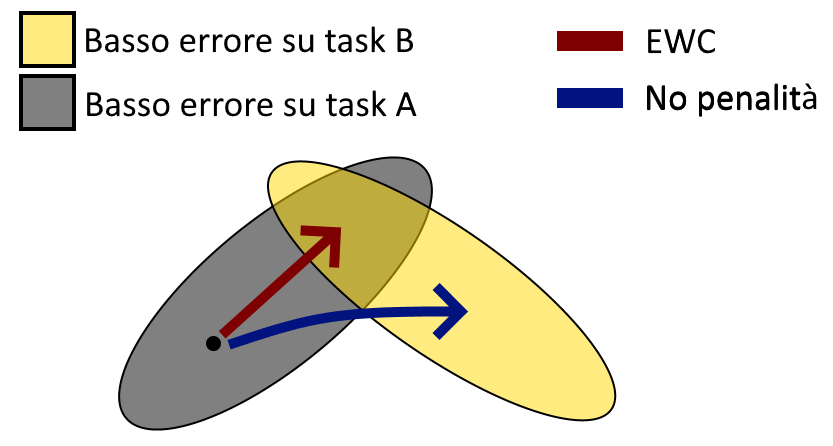
\includegraphics[width=0.5\textwidth]{img/ewc.png}
		\caption{Schematizzazione del comportamento di EWC}
		\label{fig:ewc}
	\end{center}
\end{figure}
% Implementazione: \cite{moriarty_ewc}
\subsection{Learning Without Forgetting}
La metodologia Learning Without Forgetting, delineata nell'omonima pubblicazione$^{\cite{li2017learning}}$, sfrutta esclusivamente i nuovi dati per addestrare il modello mantenendo la conoscenza già appresa.\\
Questo metodo parte da una rete che possiede parametri $\Theta$, di cui i parametri $\Theta_s$ sono condivisi fra i task e i parametri $\Theta_A$ sono specifici al task $A$. L'obiettivo è aggiungere parametri $\Theta_B$ per il nuovo task usando solo i nuovi dati senza deteriorare la conoscenza precedentemente appresa.\\\\
LWF inizia applicando il modello addestrato ai dati nuovi appena arrivati, registrando i risultati che esso produce. Dopodiché si addestra il modello, usando come loss la somma di due loss così definite:
\begin{equation}\label{eq:lwf_lossnew}
    loss_{new}(y_n, \overline{y}_n) = -y_n\cdot\log\overline{y}_n
\end{equation}
\begin{equation}\label{eq:lwf_lossnew}
    loss_{old}(y_o, \overline{y}_o) = -\sum_{i=1}^l y_o^{'(i)}\log y_o^{'(i)}
\end{equation}
dove
\begin{equation}\label{eq:lwf_lossnew}
    y_o^{'(i)} = \frac{\left(y_o^{(i)}\right)^{1/T}}{\sum_j \left(y_o^{(j)}\right)^{1/T}},\:\:\:\:\:
    \overline{y}_o^{'(i)} = \frac{\left(\overline{y}_o^{(i)}\right)^{1/T}}{\sum_j \left(\overline{y}_o^{(j)}\right)^{1/T}}
\end{equation}
$T$ è un parametro della \textit{Knowledge Distillation loss} settato a $T = 2$, $l$ è il numero di etichette, $y_n$ le etichette dei nuovi dati, $\overline{y}_n$ le predizioni dei nuovi dati, $y_o$ le precedenti previsioni del precedente modello e $\overline{y}_o$ le nuove previsioni del precedente modello.\\
La nuova loss è quindi
\begin{equation}\label{eq:lwf_loss}
    \lambda_o\cdot loss_{old}(Y_o, \overline{Y}_o) + loss_{new}(Y_n, \overline{Y}_n) + R(\Theta_s, \Theta_o, \Theta_n)
\end{equation}
Dove $\lambda_o$ è un peso che è tanto più grande quanto più sono importanti i vecchi dati rispetto ai nuovi, e $R$ è una funzione di regolarizzazione dei parametri.\\\\
Questa metodologia, che tiene di conto della performance che il modello aveva fino all'arrivo dei nuovi dati, tende quindi a mantenere la rete neurale simile a quella già addestrata, evitando così di variare considerevolmente i pesi distanziandoli da quelli appresi sui dati precedenti.
\section{Conclusione}
La scelta delle metodologie adottate, elemento centrale di questa tesi, si è rivelata particolarmente laboriosa. Anzitutto si è reso necessario inquadrare precisamente lo scopo del lavoro, cioè la comparazione fra diverse tecniche di addestramento continuo applicate a dati relativi allo human state monitoring. Questo ha richiesto la selezione di dataset appropriati e in seguito la scelta di semplici metodologie di addestramento continuo che potessero essere comparate. Il confronto ha quindi richiesto la ricerca e la scelta di metriche che ne misurassero i diversi aspetti di trasferimento della conoscenza e dell'accuratezza media e finale, oltre che i tempi di addestramento e la memoria utilizzata.\\
Il tutto è stato preceduto dalla ricerca e dallo studio personale dell'argomento, oltre che dalla scelta del linguaggio, delle librerie e dell'ambiente di sviluppo. Questo ha portato ad una lunga serie di esperimenti esplorativi, per poter studiare e testare i vari aspetti del Machine Learning e delle reti neurali prima, e dell'addestramento continuo successivamente. Questi esperimenti hanno permesso di affrontare le diverse problematiche comuni ad un problema di Machine Learning: il preprocessing dei dati, l'individuazione degli iperparametri adatti ad un modello, la corretta progettazione di una rete neurale, i tempi di addestramento e altri ancora.\\\\
Tutto questo lavoro è confluito in una serie di esperimenti finali che hanno prodotto i risultati presentati nel prossimo capitolo.

% Aggiungere queste parti? \/
% Esperimenti
% Magari racconto velocemente i diversi metodologie e difficoltà errori riscontrati?
% dovrei parlare di tutti i tentativi ed esperimenti da giugno a ora o solamente degli metodologie "finali" adottati?
% inizialmente: studio su come realizzare le reti neurali, esperimenti personali per familiarizzare con API
% poi inizio studio su come affrontare il training...

% --> capitolo successivo, Risultati